\section{Theoretical Analysis}
\label{sec:analysis}

In this section, the circuit shown in Figure~\ref{fig:circuito} is analysed
theoretically, this is, we will be using both the mesh method and the nodal method to calculate the remaining variables ($I_b$, $I_c$, $V_b$ and $V_c$).

\subsection{Mesh Method}

By using Mesh method or loop analysis we analyzed the given circuit splitting it in four meshes with the currents $I_a$ $I_b$ $I_c$ and $I_d$ (given). The direction of each mesh’s current is shown below:

\begin{figure}[H] \centering
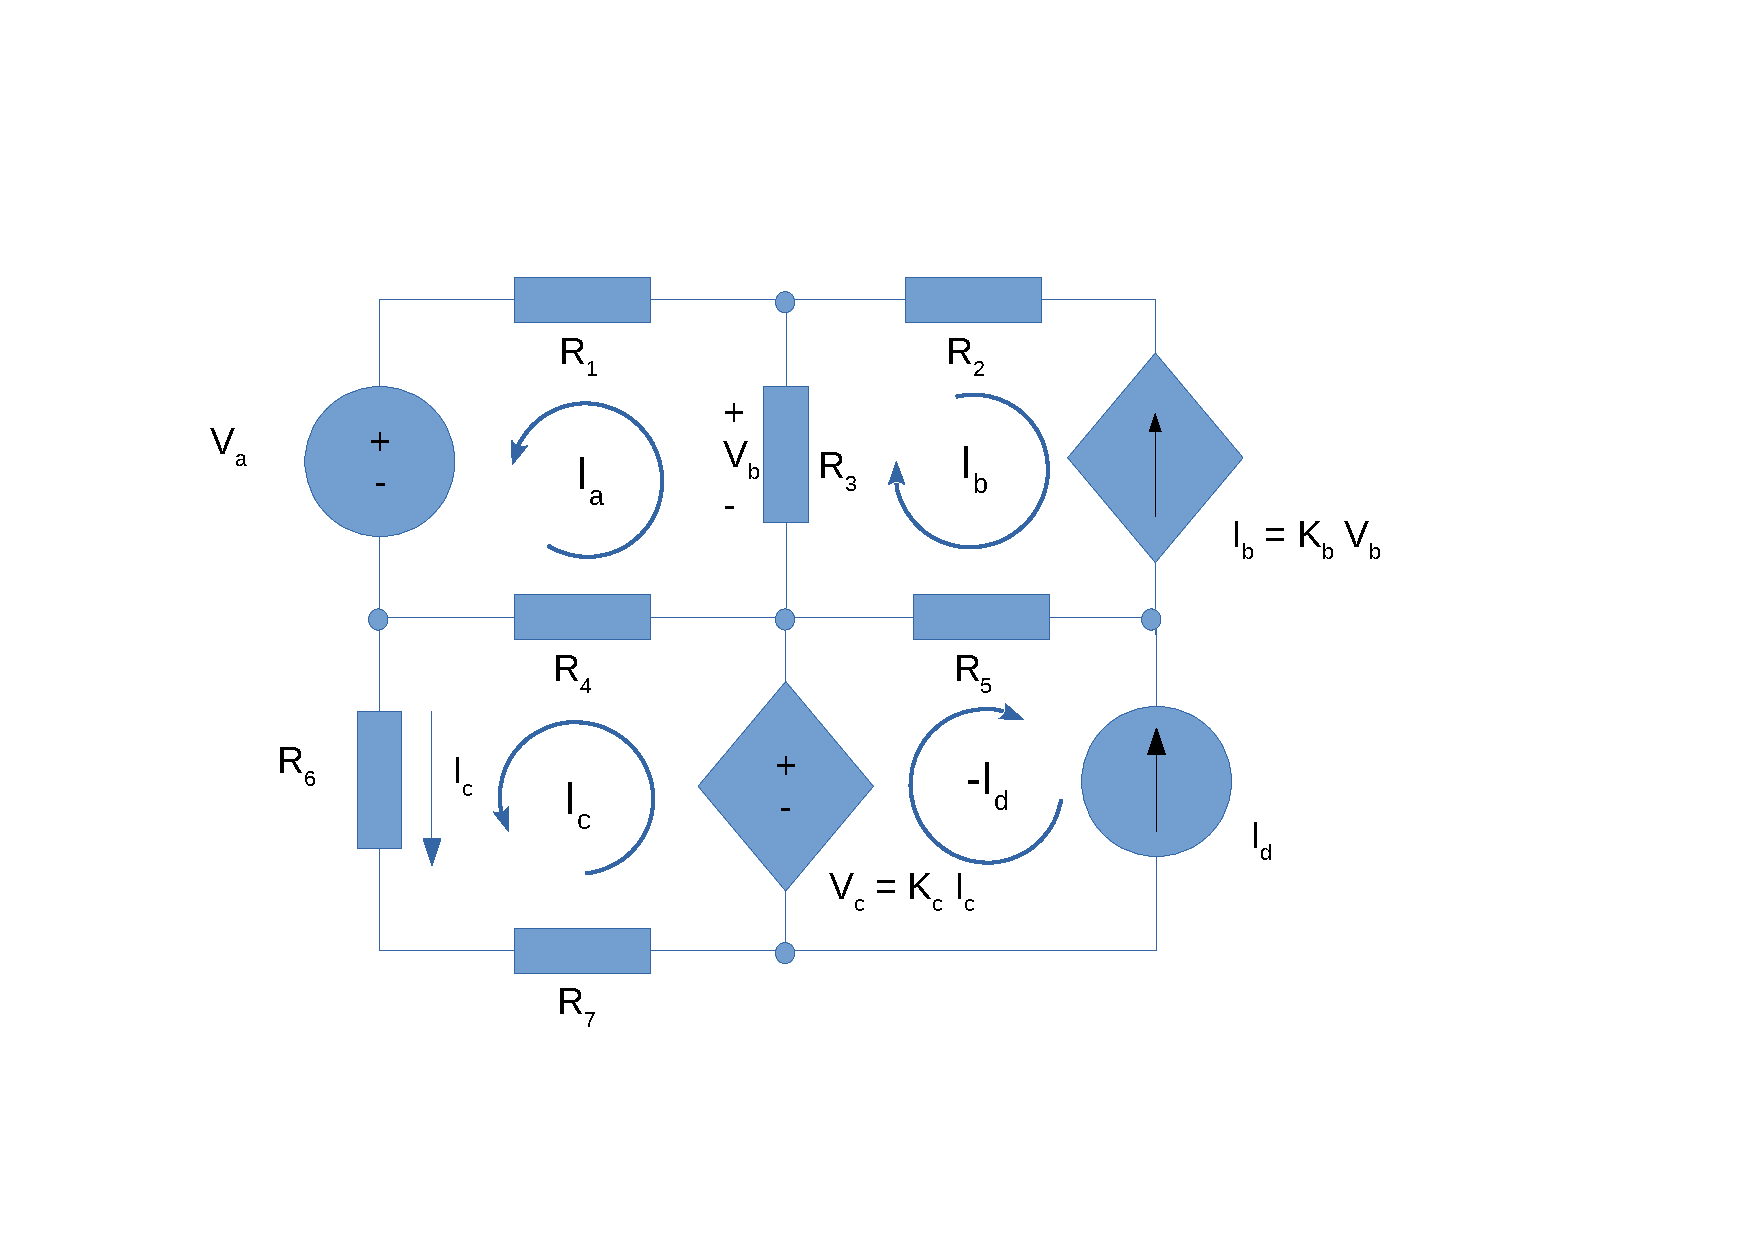
\includegraphics[width=0.7\linewidth]{malhas.pdf}
\caption{Mesh method circuit.}
\label{fig:malhas}
\end{figure}

It’s important to mention that in resistors $R_3$ and $R_5$ there is the current contribution from two meshes at the same time, as it is shown in the two following equations. \par
For mesh A, we have:
\begin{equation}
  V_a = I_a (R_1+R_4)-I_c R_4 + V_b
  \label{eq1}
\end{equation}
For mesh C, we have:
\begin{equation}
  I_a R_4 - I_c (R_4+R_6+R_7) + V_c = 0
  \label{eq2}
\end{equation}
And then, we have used additional equations, such as:
\begin{equation}
  V_c = I_c K_c
  \label{eq3}
\end{equation}

\begin{equation}
  I_b = V_b K_b
  \label{eq4}
\end{equation}

\begin{equation}
  V_b = R_3 (I_a+I_b)
  \label{eq5}
\end{equation}
Both the equations 3 and 4 are given in the original circuit figure. \par
Using these equations described above, we wrote a simple Octave script so that we could get the remaining values to fully describe the circuit. \par
The results we got using the mesh method were the following: 
\begin{center}
  \begin{tabular}{ | c | c | }
    \hline    
    {\bf Name} & {\bf Value [A or V]} \\ \hline
    $V_b$ & -4.128985e-02 \\ \hline 
$V_c$ & -7.556414e+00 \\ \hline 
$I_b$ & -3.006765e-04 \\ \hline 
$I_c$ & -9.031846e-04 \\ 

    \hline
  \end{tabular}
\end{center}
All the variables preceded by I are currents and are expressed in Ampere, the other variables, preceeded by V are voltages and are expressed in Volt.

\subsection{Nodal Method}

This method is characterized as a powerful method to compute by using matrix analysis in octave or matlab. Nodal Voltage Analysis uses the nodal equations of Kirchhoff’s first law to find the voltage potentials around the circuit. The nodes numeration is shown below:

\begin{figure}[H] \centering
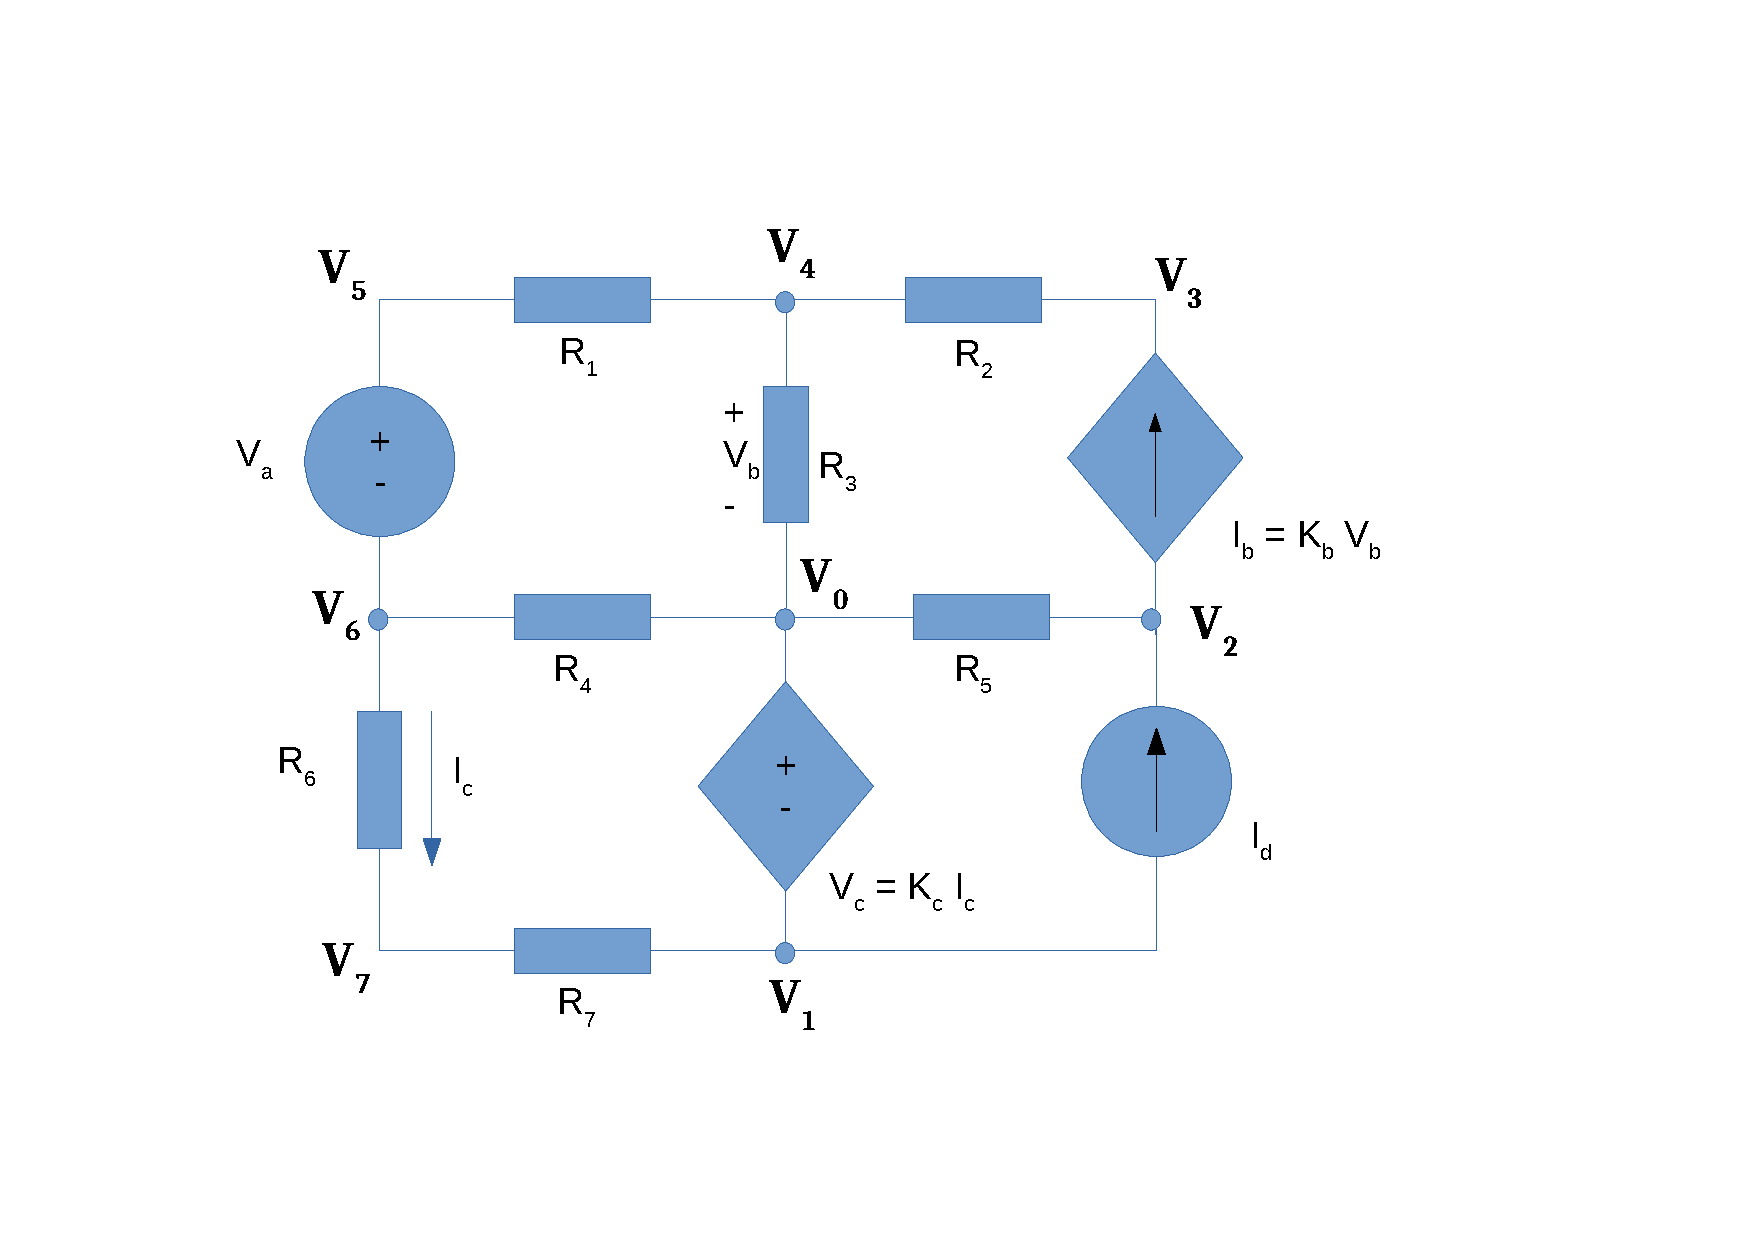
\includegraphics[width=0.7\linewidth]{nos.pdf}
\caption{Nodal method circuit.}
\label{fig:nos}
\end{figure}

The equations used to solve the system were the following:

\begin{equation}
  \frac{1}{R_2} (V_3-V_4) + \frac{1}{R_1} (V_5-V_4) - V_b \frac{1}{R_3} = 0
  \label{eq6}
\end{equation}

\begin{equation}
  \frac{1}{R_2} (V_4-V_3) + I_b = 0
  \label{eq7}
\end{equation}

\begin{equation}
  \frac{1}{R_5} (V_0-V_2) - I_b = -I_d
  \label{eq8}
\end{equation}

\begin{equation}
  \frac{1}{R_6} (V_6-V_7) - I_c = 0
  \label{eq9}
\end{equation}

We also used the following additional equations, as the previous were not enough to solve all the variables.

\begin{equation}
  V_0 = 0
  \label{eq10}
\end{equation}

\begin{equation}
  V_5 - V_6 = V_a
  \label{eq11}
\end{equation}

\begin{equation}
  V_b - K_c I_c = 0
  \label{eq12}
\end{equation}

\begin{equation}
  -V_0 + V_4 - V_b = 0
  \label{eq13}
\end{equation}

\begin{equation}
  \frac{1}{R_7} (V_1-V_7) + I_c = 0
  \label{eq14}
\end{equation}

\begin{equation}
  -V_b K_b + I_b = 0
  \label{eq15}
\end{equation}

\begin{equation}
  \frac{1}{R_4} (V_0-V_6) + \frac{1}{R_1} (V_4-V_5) - I_c = 0
  \label{eq16}
\end{equation}

\begin{equation}
  V_0 - V_1 - V_c = 0
  \label{eq17}
\end{equation}

Similarly to the mesh method we used a simple Octave script to calculate the remaining variables, the results we got using the nodal method were the following: 

\begin{center}
  \begin{tabular}{ | c | c | }
    \hline    
    {\bf Name} & {\bf Value [A or V]} \\ \hline
    $V_b$ & -4.128985e-02 \\ \hline 
$V_c$ & 7.556414e+00 \\ \hline 
$I_b$ & -3.006765e-04 \\ \hline 
$I_c$ & 9.031846e-04 \\ 

    \hline
  \end{tabular}
\end{center}
All the variables preceded by I are currents and are expressed in Ampere, the other variables, preceeded by V are voltages and are expressed in Volt.




